
%(BEGIN_QUESTION)
% Copyright 2007, Tony R. Kuphaldt, released under the Creative Commons Attribution License (v 1.0)
% This means you may do almost anything with this work of mine, so long as you give me proper credit

Shown here is the response of a process to a series of step-changes on the controller output (all made with the controller in ``manual'' mode).  Based on your observations, what can you ascertain about the process and its related instrumentation?

$$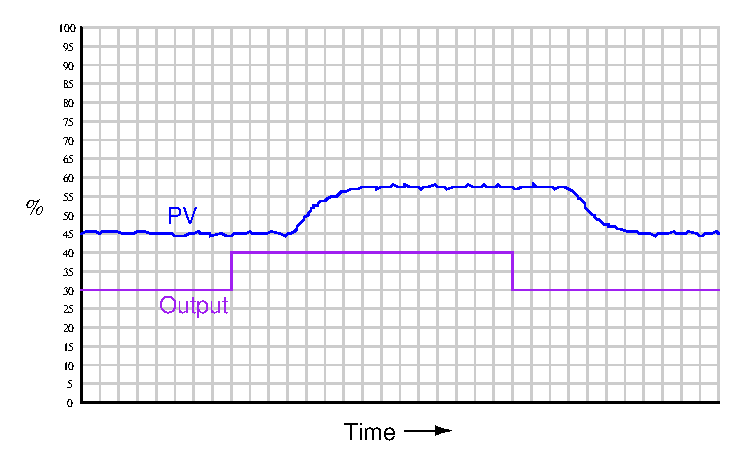
\includegraphics[width=15.5cm]{i01650x01.eps}$$

Also, calculate the {\it steady-state gain} ($K$) of this process, based on the trend shown above.

\underbar{file i01650}
%(END_QUESTION)





%(BEGIN_ANSWER)

This plot of PV response for several step-changes in output shows the process to possess a significant amount of {\it dead time}, technically known as {\it transport delay}.  There are many potential causes of dead time, but the most common is poor location of the primary sensing element (PSE), so that a significant amount of time must elapse before the process flow carries the result of the final control element's change to the sensor.  An example of this is temperature control on items carried by a conveyor belt, with the temperature sensor and heating element located far apart from each other on the belt: 

$$\includegraphics[width=15.5cm]{i01650x02.eps}$$

Other possibilities exist, however.  For instance, this phenomenon may also be produced by a combination of stiction and limited air flow in a pneumatic valve actuator.

\vskip 10pt

The {\it steady-state gain} of a self-regulating process is defined as the change in process variable ($\Delta$PV) resulting from a change in manipulated variable ($\Delta$Output).  In this case, a 10\% step-change in output produced approximately 12.5\% of change in the process variable (from about 45\% to about 57.5\%): a ratio of 1.25.

\vskip 10pt

$K$ = 1.25 (approximately)

%(END_ANSWER)





%(BEGIN_NOTES)


%INDEX% Control, PID tuning: step change (output) revealing hysteresis

%(END_NOTES)


